\documentclass[11pt,a4paper]{article}

\usepackage[utf8]{inputenc}
\usepackage[T1]{fontenc}
\usepackage{amsmath,amssymb,amsthm,mathtools,thmtools}
\usepackage{tikz}
\usetikzlibrary{arrows.meta,calc,positioning,decorations.markings,3d,patterns,fit,shapes.geometric}
\usepackage{tikz-cd}
\usepackage{pgfplots}\pgfplotsset{compat=1.18}
\usepackage{geometry}\geometry{margin=2.5cm}
\usepackage{hyperref}
\hypersetup{colorlinks=true,linkcolor=blue!60!black,citecolor=green!40!black,urlcolor=blue!50!black}
\usepackage{xurl}
\usepackage[capitalise,noabbrev]{cleveref}
\usepackage{enumitem}
\usepackage{booktabs}
\usepackage{array}
\usepackage{float}
\usepackage{algorithm}
\usepackage{algpseudocode}
\usepackage{xcolor}
\usepackage{microtype}

% Théorèmes
\theoremstyle{plain}
\newtheorem{theorem}{Theorem}[section]
\newtheorem{proposition}[theorem]{Proposition}
\newtheorem{lemma}[theorem]{Lemma}
\newtheorem{corollary}[theorem]{Corollary}
\theoremstyle{definition}
\newtheorem{definition}[theorem]{Definition}
\newtheorem{example}[theorem]{Example}
\theoremstyle{remark}
\newtheorem{remark}[theorem]{Remark}

% Macros
\newcommand{\N}{\mathbb{N}}
\newcommand{\Z}{\mathbb{Z}}
\newcommand{\R}{\mathbb{R}}
\newcommand{\Hil}{\mathcal{H}}
\newcommand{\Enc}{\mathcal{E}}
\newcommand{\Nor}{\mathcal{N}}
\newcommand{\Fc}{\mathfrak{F}}
\newcommand{\Grid}{\mathcal{G}}
\DeclareMathOperator{\card}{card}
\DeclareMathOperator{\BW}{BW}
\DeclareMathOperator{\Var}{Var}

\title{\textbf{Parametric Hilbert Volume Encoding (PHVE):\\
Bijective Encoding of Compact Reference Families,\\
with Locality, Hierarchy, and Variance Bounds}}

\author{
  Paul dit Akouni Guindo\thanks{Universit\'e Gaston Berger de Saint-Louis,
   UFR SAT D\'epartement de Math\'ematiques, B.P.~234, Saint-Louis,
   S\'en\'egal. \texttt{guindo.paul-dit-akouni@ugb.edu.sn}}
  \and
  Mamadou Abdoul Diop\thanks{Universit\'e Gaston Berger de Saint-Louis,
   UFR SAT D\'epartement de Math\'ematiques, B.P.~234, Saint-Louis,
   S\'en\'egal; UMMISCO UMI 209 IRD/UPMC, Bondy, France.
   \texttt{mamadou-abdoul.diop@ugb.edu.sn} (Corresponding author)}
}

\date{\today}

\begin{document}

\maketitle

\begin{abstract}
We introduce \emph{Parametric Hilbert Volume Encoding} (PHVE), a spatial
encoding system that establishes a bijection between discrete cells of a
$d$-dimensional grid and compact alphanumeric codes via Hilbert space-filling
curves. The system is parameterised by an arbitrary
\emph{PHVE Reference Family} $(d,\mathcal{A},\{V_\alpha\}_{\alpha\in\mathcal{A}})$
where each $V_\alpha\subset\R^d$ is a compact axis-aligned box;
the encoding map
$\Fc_p^{(d),\alpha} = \Enc_p^{(d)}\circ \Hil_p^{(d)}\circ \Nor_p^{(d),\alpha}$
sends a coordinate to a base-$29$ string over an unambiguous alphabet.

We prove bijectivity for $d\in\{2,3\}$ by structural induction on the Hilbert
recursion (\Cref{thm:bij2d,thm:bij3d}), establish forward and inverse
locality bounds (\Cref{thm:locality}), prove the hierarchy-by-truncation
property (\Cref{thm:truncation}), and derive a Lipschitz variance bound for
Differential Pulse-Code Modulation (DPCM) along the Hilbert traversal
(\Cref{thm:dpcm}). Four representative instances are given in detail:
B-tree indexation of volumetric data, Lipschitz-DPCM compression,
finite-element (FEM) mesh renumbering, and surface morphing
by Hilbert reparameterisation. A reference implementation is openly available.
\end{abstract}

\noindent\textbf{Keywords:} Hilbert curve, bijective encoding, locality bounds,
Lipschitz signals, FEM bandwidth, mesh renumbering.

\noindent\textbf{MSC 2020:} 26A16, 65N50, 68P05, 68U05, 94A29.

\section{Introduction}\label{sec:intro}

Space-filling curves were introduced by Hilbert~\cite{hilbert1891} in
1891 to exhibit a continuous surjection $H:[0,1]\to[0,1]^2$, contradicting
the geometric intuition that a line cannot fill a surface. Their
discrete counterparts were later recognised as a fundamental tool in
spatial database indexing~\cite{lawder2001}, image processing
\cite{moon2001}, and finite-element mesh ordering~\cite{cuthill1969}.
A standard reference on the subject is Sagan~\cite{sagan1994}. For a
discretisation of $[0,1]^d$ at order $p$, the Hilbert curve provides a
bijection $\mathcal{H}_p^{(d)}: \{0,\dots,2^p-1\}^d \to \{0,\dots,2^{dp}-1\}$
which preserves spatial locality optimally among space-filling
curves~\cite{niedermeier2002}.

The aim of this paper is to develop, on top of $\mathcal{H}_p^{(d)}$,
a complete \emph{encoding} pipeline that turns a point of an arbitrary
compact axis-aligned box $V\subset\R^d$ into a fixed-length string over
a finite alphabet $\Sigma$, in such a way that the resulting map enjoys
four properties simultaneously:
bijectivity onto its image (so that decoding is unambiguous);
quantitative locality preservation (so that prefixes of the code
identify spatially connected regions);
hierarchy by truncation (so that the encoding doubles as a multi-scale
spatial index); and
typographical robustness (so that the alphabet contains no pair of
visually indistinguishable symbols).
The first three are mathematical requirements; the fourth is a
practical constraint dictated by the use of the codes on physical
media. We call the resulting object \emph{Parametric Hilbert Volume
Encoding} (PHVE).

The motivation for the parametric refinement
$V \to V_\alpha$, where $\alpha$ ranges over a finite label set
$\mathcal{A}$, is that real applications work with several reference
domains rather than a single normalised cube. In medical imaging, for
instance, anatomical regions (cranium, thorax, abdomen) have distinct
nominal extents; in geographic addressing, each country admits its own
bounding box; in finite-element analysis, each computational sub-domain
has its own bounding box. We accordingly define a \emph{PHVE Reference
Family} as a triple
$(d,\mathcal{A},\{V_\alpha\}_{\alpha\in\mathcal{A}})$ and parameterise
the encoding map by $\alpha$.

Several encoding systems used in practice address part of the same
problem. Geohash~\cite{niemeyer2008} relies on a Z-order (Morton)
traversal: it is bijective and hierarchical but its locality is poor,
in the sense that two $L^\infty$-adjacent grid cells may share an
empty common prefix. Plus Codes~\cite{google2014} provide a hierarchical
$d=2$ grid but no quantitative locality bound. What3Words is bijective
but neither locality-preserving nor hierarchical. None of these systems
is parametric over a family of reference domains, nor does any extend
naturally to $d=3$. On the algorithmic side, efficient procedures for
the integer-to-index map $\mathcal{H}_p^{(d)}$ itself have been given
by Butz~\cite{butz1971}, Liu and Schrack~\cite{liu1996}, and
Skilling~\cite{skilling2004}; these works treat $\mathcal{H}_p^{(d)}$
in isolation and do not address the encoding pipeline considered here.

The basic idea of the present paper is to factor the encoding map as
$\mathfrak{F}_p^{(d),\alpha} = \mathcal{E}_p^{(d)} \circ
\mathcal{H}_p^{(d)} \circ \mathcal{N}_p^{(d),\alpha}$, where
$\mathcal{N}_p^{(d),\alpha}$ is the affine normalisation
$V_\alpha \to \{0,\dots,2^p-1\}^d$ specific to each reference box,
$\mathcal{H}_p^{(d)}$ is the classical Hilbert bijection, and
$\mathcal{E}_p^{(d)}$ writes integers in base $B = |\Sigma|$ over a
$29$-symbol alphabet free of typographical ambiguity. The four
properties listed above are then established as theorems on this
factorised map: bijectivity for $d\in\{2,3\}$ (\Cref{thm:bij2d,thm:bij3d}),
forward and inverse locality bounds (\Cref{thm:locality}), hierarchy
by truncation with explicit diameter estimate (\Cref{thm:truncation}),
and a Lipschitz variance bound for differential pulse-code modulation
(DPCM) along the Hilbert traversal (\Cref{thm:dpcm}). The framework
is then instantiated on four representative applications: B-tree
indexation of volumetric data (\Cref{prop:btree}), DPCM compression of
$d$-dimensional Lipschitz signals (\Cref{sec:app_dpcm}), finite-element
mesh renumbering with bandwidth reduction (\Cref{thm:bandwidth}), and
surface morphing by Hilbert reparameterisation
(\Cref{prop:morphing}).

We emphasise that no claim of novelty is made for the integer-to-index
map $\mathcal{H}_p^{(d)}$ itself, which is classical. The contribution
of the paper lies in the construction and analysis of the parametric
encoding $\mathfrak{F}_p^{(d),\alpha}$ as a whole, in the explicit
constants we keep throughout the locality and DPCM bounds, and in the
four instantiated applications.

The paper is organised as follows. \Cref{sec:framework} sets up the
mathematical framework: alphabet, Reference Family, encoding map, and
its invariance under axis-preserving signed permutations.
\Cref{sec:hilbert} recalls the recursive constructions of the Hilbert
curve in dimensions $d=2$ and $d=3$, the latter following Skilling.
\Cref{sec:bijectivity,sec:locality,sec:truncation,sec:error} establish
the four foundational properties of $\mathfrak{F}_p^{(d),\alpha}$.
\Cref{sec:dpcm} proves the Lipschitz variance bound for DPCM along
the Hilbert traversal. \Cref{sec:algorithms} discusses the encoding
and decoding algorithms and their complexity. \Cref{sec:applications}
treats the four instantiated applications. \Cref{sec:experiments}
reports numerical validation on the MNI152 brain template, including
a deliberately disclosed negative result for DPCM compression on
heavily averaged signals. \Cref{sec:comparison} compares PHVE with
existing encoding systems, and \Cref{sec:conclusion} concludes.

\section{Mathematical Framework}\label{sec:framework}

\subsection{The Unambiguous Alphabet \texorpdfstring{$\Sigma$}{Sigma}}
\label{sec:framework_alphabet}

\begin{definition}[Unambiguous alphabet]\label{def:alphabet}
We define the alphabet
\[
\Sigma = \{2,3,4,5,6,7,8,9,A,B,C,D,E,F,G,H,J,K,M,N,P,Q,R,S,T,V,W,X,Y\},
\]
of cardinality $B := |\Sigma| = 29$. The seven excluded characters
$\{0,O,1,I,L,U,Z\}$ are those subject to visual confusion in standard
typefaces (e.g.\ Helvetica, Arial, Times New Roman).
\end{definition}

\subsection{The PHVE Reference Family}
\label{sec:framework_family}

\begin{definition}[PHVE Reference Family]\label{def:phve_family}
A \emph{PHVE Reference Family} is a triple
$(d,\mathcal{A},\{V_\alpha\}_{\alpha\in\mathcal{A}})$ where:
\begin{itemize}[nosep]
\item $d\in\N^*$ is the spatial dimension;
\item $\mathcal{A}$ is a finite set of \emph{labels};
\item for each $\alpha\in\mathcal{A}$, $V_\alpha\subset\R^d$ is a
non-degenerate compact axis-aligned box
\[
V_\alpha = \prod_{i=1}^d [a_i^\alpha,\,b_i^\alpha],\qquad
a_i^\alpha < b_i^\alpha\text{ for all }i.
\]
\end{itemize}
\end{definition}

\begin{example}[Anatomical reference family, $d=3$]
\label{ex:anatomical}
$\mathcal{A}_0 = \{\mathtt{CR},\mathtt{TX},\mathtt{CA},\mathtt{AB},\mathtt{FB}\}$
with the dimensions of \Cref{tab:reference_volumes}. Each $V_\alpha$ is a
nominal anatomical bounding box used in clinical imaging.
\end{example}

\begin{table}[!htbp]
\centering
\small
\begin{tabular}{cll}
\toprule
Prefix & Region & Dimensions (mm) \\
\midrule
\texttt{CR} & Cranium & $300 \times 250 \times 250$ \\
\texttt{TX} & Thorax & $400 \times 350 \times 300$ \\
\texttt{CA} & Cardiac & $150 \times 120 \times 100$ \\
\texttt{AB} & Abdomen & $400 \times 350 \times 300$ \\
\texttt{FB} & Full body & $2000 \times 600 \times 400$ \\
\bottomrule
\end{tabular}
\caption{Anatomical reference family $\mathcal{A}_0$ used in
\Cref{ex:anatomical}.}
\label{tab:reference_volumes}
\end{table}

\begin{example}[Geographic reference family, $d=2$]\label{ex:geographic}
$\mathcal{A}$ is the set of ISO~3166-1 alpha-2 country codes; each
$V_\alpha\subset\R^2$ is the bounding box of a country in geodetic
coordinates $(\varphi,\lambda)$ projected to a planar chart on which
$V_\alpha$ is approximated by a rectangle. The local-flat
approximation suffices for countries of moderate extent; an extension
to a spherical reference family on $S^2$ falls outside the scope of
the present paper.
\end{example}

\begin{example}[FEM domain reference family, $d\in\{2,3\}$]
\label{ex:fem}
$\mathcal{A}$ is a singleton or a partition of a computational mesh into
sub-domains, and each $V_\alpha$ is the axis-aligned bounding box of the
corresponding sub-mesh.
\end{example}

\subsection{The Encoding Map \texorpdfstring{$\Fc_p^{(d),\alpha}$}{F}}
\label{sec:framework_encoding}

For $p\in\N^*$ we set $n=2^p$ and write
$\Grid_p^{(d)} = \{0,\dots,n-1\}^d$ for the discrete grid with $n^d$ cells.

\begin{definition}[Code length]\label{def:codelen}
The number of base-$B$ symbols required to represent any index in
$\{0,\dots,n^d-1\}$ is
\[
k_d(p) := \left\lceil \dfrac{d\,p\,\ln 2}{\ln B} \right\rceil.
\]
\end{definition}

\begin{definition}[Encoding map]\label{def:encoding_map}
For a PHVE Reference Family $(d,\mathcal{A},\{V_\alpha\})$, an order
$p\in\N^*$ and a label $\alpha\in\mathcal{A}$, the encoding map is the
composition
\[
\Fc_p^{(d),\alpha} := \Enc_p^{(d)} \circ \Hil_p^{(d)} \circ \Nor_p^{(d),\alpha},
\]
where
\begin{itemize}[nosep]
\item the \emph{normalisation}
$\Nor_p^{(d),\alpha}: V_\alpha \to \Grid_p^{(d)}$ is given by
\[
\Nor_p^{(d),\alpha}(\mathbf{x})_i = \min\!\Bigl(n-1,\,
\Bigl\lfloor \dfrac{x_i - a_i^\alpha}{b_i^\alpha - a_i^\alpha}\,n
\Bigr\rfloor\Bigr),\quad i=1,\dots,d;
\]
\item the \emph{Hilbert bijection}
$\Hil_p^{(d)}:\Grid_p^{(d)}\to \{0,\dots,n^d-1\}$ is defined recursively
in~\Cref{sec:hilbert};
\item the \emph{base-$B$ injection}
$\Enc_p^{(d)}: \{0,\dots,n^d-1\}\hookrightarrow \Sigma^{k_d(p)}$
sends an integer to its zero-padded representation in $\Sigma$.
\end{itemize}
\end{definition}

% Wrapper holding the placement of the commutative diagram.
\begin{figure}[!htbp]
  \centering
  % Figure 1 (logical Figure 3): commutative diagram of F = E o H o N.
% Two-row layout: forward maps top, inverses bottom.
\begin{tikzcd}[
  ampersand replacement=\&,
  column sep=3.6em,
  row sep=2.8em,
  every label/.append style={font=\footnotesize}
]
V_\alpha \arrow[r, "\Nor_p^{(d),\alpha}"]
\& \Grid_p^{(d)} \arrow[r, "\Hil_p^{(d)}"]
\& \{0,\dots,n^d{-}1\} \arrow[r, "\Enc_p^{(d)}"]
\& \Sigma^{k_d(p)} \\
V_\alpha
\& \Grid_p^{(d)}
   \arrow[l, dashed, "(\Nor_p^{(d),\alpha})^{-1}"']
\& \{0,\dots,n^d{-}1\}
   \arrow[l, dashed, "(\Hil_p^{(d)})^{-1}"']
\& \Sigma^{k_d(p)}
   \arrow[l, dashed, "(\Enc_p^{(d)})^{-1}"']
\end{tikzcd}

  \caption{The encoding map
  $\Fc_p^{(d),\alpha} = \Enc_p^{(d)} \circ \Hil_p^{(d)} \circ \Nor_p^{(d),\alpha}$
  visualised as a two-row diagram. \emph{Top row:} the three forward maps
  composed left-to-right; their composition is $\Fc_p^{(d),\alpha}$.
  \emph{Bottom row:} the three inverses, each defined on the image of
  the corresponding forward map; their composition is
  $(\Fc_p^{(d),\alpha})^{-1} = (\Nor_p^{(d),\alpha})^{-1}
  \circ (\Hil_p^{(d)})^{-1} \circ (\Enc_p^{(d)})^{-1}$.}
  \label{fig:commutative}
\end{figure}


\subsection{Invariance under Axis-Preserving Isometries}
\label{sec:framework_invariance}

Let $G_d := \Z_2^d \rtimes S_d$ be the group of \emph{signed permutations}
of $\R^d$, acting on $\mathbf{x}\in\R^d$ by
$(\epsilon,\sigma)\cdot \mathbf{x} = (\epsilon_1 x_{\sigma(1)},\dots,
\epsilon_d x_{\sigma(d)})$
with $\epsilon\in\{\pm 1\}^d$ and $\sigma\in S_d$. We say a Reference
Family is \emph{$G_d$-equivariant} if for every $(\epsilon,\sigma)\in G_d$
there exists a bijection
$\tau_{\epsilon,\sigma}:\mathcal{A}\to\mathcal{A}$ such that
$V_{\tau_{\epsilon,\sigma}(\alpha)}=(\epsilon,\sigma)\cdot V_\alpha$ as
sets in $\R^d$ (after coordinate-wise reordering of bounds).

\begin{lemma}[Equivariance of the encoding]\label{lem:equivariance}
Let $(d,\mathcal{A},\{V_\alpha\})$ be a $G_d$-equivariant Reference
Family and let $g=(\epsilon,\sigma)\in G_d$. There exists a permutation
$\rho_g$ of $\Sigma^{k_d(p)}$ such that, for all $\alpha\in\mathcal{A}$
and $\mathbf{x}\in V_\alpha$,
\[
\Fc_p^{(d),\tau_g(\alpha)}(g\cdot \mathbf{x})
=\rho_g\bigl(\Fc_p^{(d),\alpha}(\mathbf{x})\bigr).
\]
\end{lemma}

\begin{proof}
The normalisation $\Nor_p^{(d),\alpha}$ commutes with $g$ on
$\Grid_p^{(d)}$ up to the obvious relabelling:
\[
\Nor_p^{(d),\tau_g(\alpha)}(g\cdot \mathbf{x})
= g\cdot \Nor_p^{(d),\alpha}(\mathbf{x}),
\]
where the $g$-action is restricted to integer signed permutations of
the cube $\Grid_p^{(d)}$. The Hilbert bijection conjugated by such a
signed permutation differs from the original by a fixed permutation
$\pi_g$ of $\{0,\dots,n^d-1\}$ (the action of $g$ on the orientation
table). The base-$B$ map $\Enc_p^{(d)}$ then transports $\pi_g$ to a
permutation $\rho_g$ of $\Sigma^{k_d(p)}$.
\end{proof}

\section{The Hilbert Curve: Recursive Construction}\label{sec:hilbert}

\subsection{Two-dimensional Construction}\label{sec:hilbert_2d}

The Hilbert curve of order $p\geq 1$ in dimension $d=2$ is the bijection
$\Hil_p^{(2)}:\Grid_p^{(2)}\to\{0,\dots,4^p-1\}$ defined recursively as follows.

\paragraph{Base case ($p=1$).} The map sends
$(0,0)\mapsto 0,\ (0,1)\mapsto 1,\ (1,1)\mapsto 2,\ (1,0)\mapsto 3$,
yielding a U-shape in the $2\times 2$ grid (\Cref{fig:hilbert2d}, left).

\paragraph{Recursive case.} Let $m = 2^{p-1}$ and write
$(r_x,r_y)=(\lfloor x/m \rfloor,\lfloor y/m \rfloor)\in\{0,1\}^2$ to identify
the quadrant containing $(x,y)$. Set
\[ q := 3 r_x \oplus r_y \in \{0,1,2,3\}, \]
where $\oplus$ denotes bitwise XOR. Then
\begin{equation}\label{eq:hilbert2d}
\Hil_p^{(2)}(x,y) = q\cdot m^2 +
\Hil_{p-1}^{(2)}\bigl(\rho_q(x \bmod m,\, y \bmod m)\bigr),
\end{equation}
where $\rho_q$ is the involutive transformation of $\{0,\dots,m-1\}^2$
defined by:
\[
\rho_q(u,v) =
\begin{cases}
(v, u) & q = 0,\\
(u, v) & q = 1,\\
(u, v) & q = 2,\\
(m{-}1{-}v,\,m{-}1{-}u) & q = 3.
\end{cases}
\]

\begin{figure}[!htbp]
  \centering
  % Figure 1: Hilbert 2D construction at orders p=1, 2, 3.
% Hilbert paths generated with the standard d2xy algorithm.
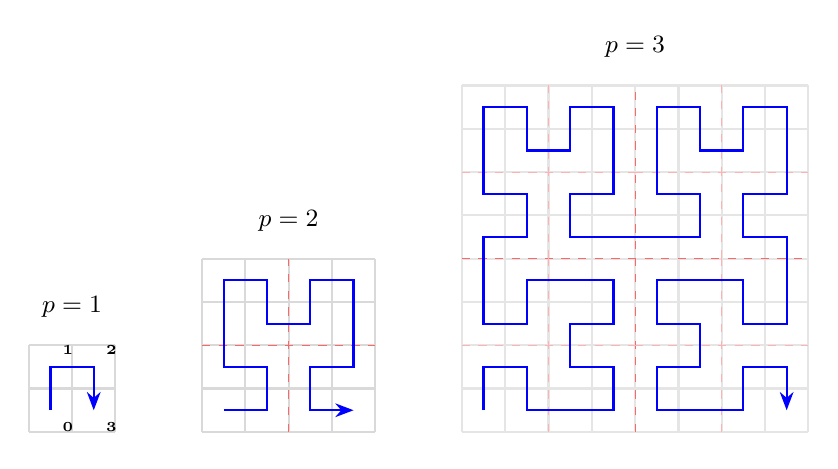
\begin{tikzpicture}[scale=0.55,>=Stealth,thick]

% --- p=1 ---
\begin{scope}[xshift=0cm]
  \node[above,font=\small] at (1,2.4) {$p=1$};
  \draw[step=1,gray!30] (0,0) grid (2,2);
  \draw[blue,->] (0.5,0.5) -- (0.5,1.5) -- (1.5,1.5) -- (1.5,0.5);
  \node at (0.5,0.5) [below right=1pt,font=\tiny\bfseries] {0};
  \node at (0.5,1.5) [above right=1pt,font=\tiny\bfseries] {1};
  \node at (1.5,1.5) [above right=1pt,font=\tiny\bfseries] {2};
  \node at (1.5,0.5) [below right=1pt,font=\tiny\bfseries] {3};
\end{scope}

% --- p=2 ---
\begin{scope}[xshift=4cm]
  \node[above,font=\small] at (2,4.4) {$p=2$};
  \draw[step=1,gray!30] (0,0) grid (4,4);
  \draw[red!60,dashed,thin] (2,0)--(2,4) (0,2)--(4,2);
  \draw[blue,->]
    (0.5,0.5) -- (1.5,0.5) -- (1.5,1.5) -- (0.5,1.5) -- (0.5,2.5) -- (0.5,3.5)
    -- (1.5,3.5) -- (1.5,2.5) -- (2.5,2.5) -- (2.5,3.5) -- (3.5,3.5) -- (3.5,2.5)
    -- (3.5,1.5) -- (2.5,1.5) -- (2.5,0.5) -- (3.5,0.5);
\end{scope}

% --- p=3 ---
\begin{scope}[xshift=10cm]
  \node[above,font=\small] at (4,8.4) {$p=3$};
  \draw[step=1,gray!20] (0,0) grid (8,8);
  \draw[red!60,dashed,thin] (4,0)--(4,8) (0,4)--(8,4);
  \draw[red!30,dashed,very thin]
    (2,0)--(2,4)  (6,0)--(6,4)
    (0,2)--(4,2)  (4,2)--(8,2)
    (2,4)--(2,8)  (6,4)--(6,8)
    (0,6)--(4,6)  (4,6)--(8,6);
  \draw[blue,->]
    (0.5,0.5) -- (0.5,1.5) -- (1.5,1.5) -- (1.5,0.5) -- (2.5,0.5) -- (3.5,0.5)
    -- (3.5,1.5) -- (2.5,1.5) -- (2.5,2.5) -- (3.5,2.5) -- (3.5,3.5) -- (2.5,3.5)
    -- (1.5,3.5) -- (1.5,2.5) -- (0.5,2.5) -- (0.5,3.5) -- (0.5,4.5) -- (1.5,4.5)
    -- (1.5,5.5) -- (0.5,5.5) -- (0.5,6.5) -- (0.5,7.5) -- (1.5,7.5) -- (1.5,6.5)
    -- (2.5,6.5) -- (2.5,7.5) -- (3.5,7.5) -- (3.5,6.5) -- (3.5,5.5) -- (2.5,5.5)
    -- (2.5,4.5) -- (3.5,4.5) -- (4.5,4.5) -- (5.5,4.5) -- (5.5,5.5) -- (4.5,5.5)
    -- (4.5,6.5) -- (4.5,7.5) -- (5.5,7.5) -- (5.5,6.5) -- (6.5,6.5) -- (6.5,7.5)
    -- (7.5,7.5) -- (7.5,6.5) -- (7.5,5.5) -- (6.5,5.5) -- (6.5,4.5) -- (7.5,4.5)
    -- (7.5,3.5) -- (7.5,2.5) -- (6.5,2.5) -- (6.5,3.5) -- (5.5,3.5) -- (4.5,3.5)
    -- (4.5,2.5) -- (5.5,2.5) -- (5.5,1.5) -- (4.5,1.5) -- (4.5,0.5) -- (5.5,0.5)
    -- (6.5,0.5) -- (6.5,1.5) -- (7.5,1.5) -- (7.5,0.5);
\end{scope}

\end{tikzpicture}

  \caption{Hilbert curve in dimension $d=2$ at orders $p=1,2,3$.
  Cells are indexed by their Hilbert order; dashed lines separate
  the four sub-quadrants; arrows trace the curve $\Hil_p^{(2)}$.}
  \label{fig:hilbert2d}
\end{figure}

\subsection{Three-dimensional Construction (Skilling)}\label{sec:hilbert_3d}

In dimension $d=3$, the Hilbert curve of order $p$ partitions the cube
$\Grid_p^{(3)} = \{0,\dots,n-1\}^3$ into eight sub-cubes (\emph{octants}),
each isomorphic to $\Grid_{p-1}^{(3)}$, and traverses each by a rotated
copy of $\Hil_{p-1}^{(3)}$. The rotation table consists of eight
orientation states drawn from the wreath product
$\Z_2^3\rtimes S_3$ of signed coordinate permutations.

We adopt the algorithm of Skilling~\cite{skilling2004}, which operates
directly on the bit representation via the Gray code and a sequence of
bit-level transposes. Its pseudocode is recalled in
\Cref{alg:skilling_xyz2d}.

\begin{algorithm}[H]
\caption{Skilling 3D: coordinates to Hilbert index}\label{alg:skilling_xyz2d}
\begin{algorithmic}[1]
\Require coordinates $(x_0,x_1,x_2)\in\Grid_p^{(3)}$, order $p$
\Ensure Hilbert index $d \in \{0,\dots,8^p-1\}$
\State $M \gets 2^{p-1}$
\For{$Q = M$ down to $2$}
  \State $P \gets Q-1$
  \For{$i = 0$ to $2$}
    \If{$x_i \mathbin{\mathrm{AND}} Q \ne 0$}
      \State $x_0 \gets x_0 \oplus P$
    \Else
      \State $t \gets (x_0 \oplus x_i) \mathbin{\mathrm{AND}} P$
      \State $x_0 \gets x_0 \oplus t$;\quad $x_i \gets x_i \oplus t$
    \EndIf
  \EndFor
\EndFor
\For{$i = 1$ to $2$}
  \State $x_i \gets x_i \oplus x_{i-1}$
\EndFor
\State $t \gets 0$;\quad $Q \gets M$
\While{$Q > 1$}
  \If{$x_2 \mathbin{\mathrm{AND}} Q \ne 0$}
    \State $t \gets t \oplus (Q-1)$
  \EndIf
  \State $Q \gets Q/2$
\EndWhile
\For{$i = 0$ to $2$}
  \State $x_i \gets x_i \oplus t$
\EndFor
\State $d \gets \mathrm{Interleave}(x_0,x_1,x_2,p)$
\State \Return $d$
\end{algorithmic}
\end{algorithm}

The interleaving step combines three $p$-bit numbers into a single
$3p$-bit index:
\begin{equation}\label{eq:interleave}
\mathrm{Interleave}(x_0,x_1,x_2,p) = \sum_{i=0}^{p-1}
\bigl[ x_0^{(i)} 2^{3i+2} + x_1^{(i)} 2^{3i+1} + x_2^{(i)} 2^{3i} \bigr],
\end{equation}
where $x_j^{(i)}$ denotes the $i$-th bit of $x_j$.

\begin{lemma}[Interleave is bijective]\label{lem:interleave}
The map $\mathrm{Interleave}:\Grid_p^{(3)}\to\{0,\dots,8^p-1\}$ defined by
\eqref{eq:interleave} is a bijection.
\end{lemma}

\begin{proof}
The right-hand side of \eqref{eq:interleave} is the binary expansion of
an integer in $\{0,\dots,8^p-1\}$ written as $3p$ bits, with bits at
positions $\{3i+2,3i+1,3i\}_{i=0}^{p-1}$ taken from
$\{x_0^{(i)},x_1^{(i)},x_2^{(i)}\}$ respectively. Inverting bit by bit
recovers each $x_j$ uniquely; the resulting map
$\{0,\dots,8^p-1\}\to\Grid_p^{(3)}$ is a two-sided inverse.
\end{proof}

\begin{figure}[!htbp]
  \centering
  % Figure 2: Hilbert 3D order p=2 with octant centres path.
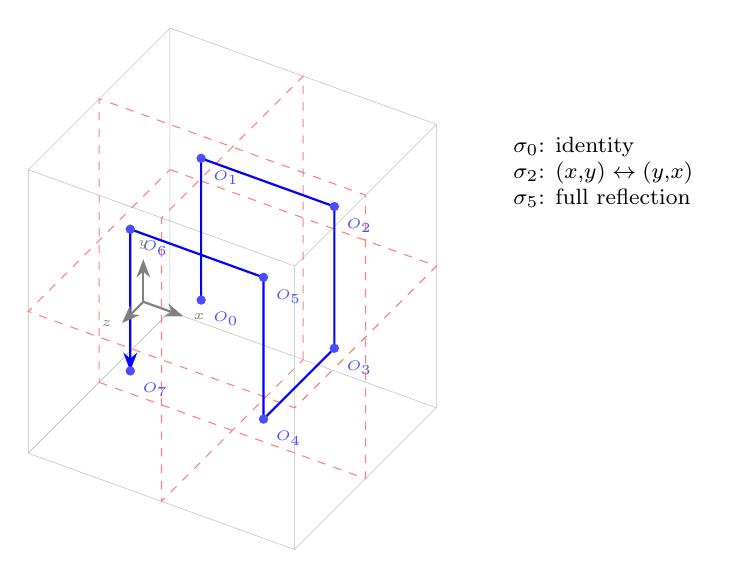
\begin{tikzpicture}[
  scale=0.9,
  >=Stealth,
  thick,
  every node/.style={font=\footnotesize},
  x  ={(0.94cm,-0.34cm)},
  y  ={(0cm,1cm)},
  z  ={(-0.5cm,-0.5cm)}]

% --- Outer cube (p=2 means side = 4) ---
\draw[gray!50,very thin]
  (0,0,0) -- (4,0,0) -- (4,4,0) -- (0,4,0) -- cycle
  (0,0,4) -- (4,0,4) -- (4,4,4) -- (0,4,4) -- cycle
  (0,0,0) -- (0,0,4)  (4,0,0) -- (4,0,4)
  (4,4,0) -- (4,4,4)  (0,4,0) -- (0,4,4);

% --- Three mid-planes separating octants ---
\draw[red!50,dashed,thin]
  (2,0,0) -- (2,4,0) -- (2,4,4) -- (2,0,4) -- cycle
  (0,2,0) -- (4,2,0) -- (4,2,4) -- (0,2,4) -- cycle
  (0,0,2) -- (4,0,2) -- (4,4,2) -- (0,4,2) -- cycle;

% --- Hilbert path through 8 octant centres (canonical Skilling order) ---
\draw[blue,->,thick]
  (1,1,1) -- (1,3,1) -- (3,3,1) -- (3,1,1) --
  (3,1,3) -- (3,3,3) -- (1,3,3) -- (1,1,3);

% --- Octant labels at centres ---
\foreach \q/\X/\Y/\Z in {0/1/1/1, 1/1/3/1, 2/3/3/1, 3/3/1/1,
                         4/3/1/3, 5/3/3/3, 6/1/3/3, 7/1/1/3}
  \filldraw[blue!70] (\X,\Y,\Z) circle (1.4pt)
    node[below right=1pt,font=\tiny\bfseries] {$O_{\q}$};

% --- Sample orientations on the right ---
\node[align=left,anchor=west,font=\footnotesize]
  at (5.0,3.5,0) {%
  $\sigma_0$: identity\\
  $\sigma_2$: $(x{,}y) \leftrightarrow (y{,}x)$\\
  $\sigma_5$: full reflection\\
  };

% --- Coordinate axes ---
\draw[->,gray] (-0.4,0,0) -- (-0.4,0.6,0) node[above,font=\tiny] {$y$};
\draw[->,gray] (-0.4,0,0) -- (0.2,0,0) node[right,font=\tiny] {$x$};
\draw[->,gray] (-0.4,0,0) -- (-0.4,0,0.6) node[left,font=\tiny] {$z$};

\end{tikzpicture}

  \caption{Three-dimensional Hilbert curve at order $p=2$ (Skilling
  construction). The unit cube is partitioned into 8 octants; the
  centres of the octants are joined by the Hilbert path. Sample
  orientations $\sigma_q$ are listed.}
  \label{fig:hilbert3d}
\end{figure}

\section{Bijectivity Theorems}\label{sec:bijectivity}

\subsection{Two-dimensional Bijectivity}\label{sec:bij_2d}

The inductive step of the bijectivity proof rests on the following
elementary property of the rotations $\rho_q$ of~\eqref{eq:hilbert2d}.

\begin{lemma}[The rotations $\rho_q$ are involutions]
\label{lem:rho_involutive}
Let $m\geq 1$ and let $\rho_0,\rho_1,\rho_2,\rho_3$ be the maps of
\eqref{eq:hilbert2d}. For every $q\in\{0,1,2,3\}$, $\rho_q$ is an
involution of $\{0,\dots,m-1\}^2$, hence a bijection.
\end{lemma}

\begin{proof}
For $q\in\{1,2\}$, $\rho_q$ is the identity, hence trivially an
involution. For $q=0$, $\rho_0(u,v)=(v,u)$ is the coordinate
transposition, and
$\rho_0(\rho_0(u,v))=\rho_0(v,u)=(u,v)$. For $q=3$,
$\rho_3(u,v)=(m-1-v,\,m-1-u)$, and
\[
\rho_3(\rho_3(u,v))
 = \rho_3(m-1-v,\,m-1-u)
 = \bigl(m-1-(m-1-u),\,m-1-(m-1-v)\bigr)
 = (u,v).
\]
Any involution of a finite set is a bijection.
\end{proof}

\begin{theorem}[Bijectivity, $d=2$]\label{thm:bij2d}
For every $p\geq 1$ the map
$\Hil_p^{(2)}:\{0,\dots,2^p-1\}^2\to \{0,\dots,4^p-1\}$ defined by
\eqref{eq:hilbert2d} is a bijection.
\end{theorem}

\begin{proof}
We argue by strong induction on $p$.

\emph{Base case ($p=1$).} The four explicit values
$(0,0)\mapsto 0,\ (0,1)\mapsto 1,\ (1,1)\mapsto 2,\ (1,0)\mapsto 3$
exhaust the codomain $\{0,1,2,3\}$ injectively, so $\Hil_1^{(2)}$ is a
bijection.

\emph{Inductive step.} Assume $\Hil_{p-1}^{(2)}$ is a bijection. Let
$m = 2^{p-1}$ and partition $\{0,\dots,2m-1\}^2$ into the four quadrants
\[
Q_0 = \{0,\dots,m{-}1\}\times\{0,\dots,m{-}1\},\quad
Q_1 = \{0,\dots,m{-}1\}\times\{m,\dots,2m{-}1\},
\]
and similarly $Q_2,Q_3$. The map
$(x,y)\mapsto (x\bmod m,y\bmod m)$ restricts to a bijection from each
$Q_q$ to $\{0,\dots,m{-}1\}^2$.

\emph{Injectivity.} Let $(x_1,y_1)\ne (x_2,y_2)\in\{0,\dots,2m-1\}^2$
and let $q_1,q_2$ be their respective quadrants.

\emph{Case (i): $q_1\ne q_2$.} The Hilbert indices satisfy
$\Hil_p^{(2)}(x_1,y_1)\in [q_1 m^2,(q_1+1)m^2)$ and
$\Hil_p^{(2)}(x_2,y_2)\in [q_2 m^2,(q_2+1)m^2)$. These intervals are
disjoint, so the indices differ.

\emph{Case (ii): $q_1=q_2=:q$.} Their local coordinates
$(x_i\bmod m,\, y_i\bmod m)\in \{0,\dots,m-1\}^2$ differ. By
\Cref{lem:rho_involutive}, $\rho_q$ is a bijection of
$\{0,\dots,m-1\}^2$, hence
$\rho_q(x_1\bmod m,\,y_1\bmod m) \ne \rho_q(x_2\bmod m,\,y_2\bmod m)$.
By the inductive hypothesis, $\Hil_{p-1}^{(2)}$ assigns them distinct
values in $\{0,\dots,m^2-1\}$, so the full indices differ.

\emph{Surjectivity.} The domain has cardinality $4^p$ and the codomain
has cardinality $4^p$. An injective map between finite sets of equal
cardinality is bijective.
\end{proof}

\subsection{Three-dimensional Bijectivity}\label{sec:bij_3d}

\begin{theorem}[Bijectivity, $d=3$]\label{thm:bij3d}
For every $p\geq 1$ the map
$\Hil_p^{(3)}:\{0,\dots,2^p-1\}^3\to \{0,\dots,8^p-1\}$ produced by
\Cref{alg:skilling_xyz2d} is a bijection.
\end{theorem}

As in dimension two, the proof relies on two intermediate lemmas
recording the basic properties of the Skilling decomposition.

\begin{lemma}[Octant function]\label{lem:octant}
The Skilling decomposition assigns each
$\mathbf{x}\in\{0,\dots,2^p-1\}^3$ a unique octant
$q(\mathbf{x})\in\{0,\dots,7\}$ given by the most significant bit of the
Gray code of $(x_0,x_1,x_2)$, and the map $q$ partitions the grid into
eight cosets of $\{0,\dots,m-1\}^3$ where $m = 2^{p-1}$.
\end{lemma}

\begin{proof}[Proof of \Cref{lem:octant}]
The first phase of \Cref{alg:skilling_xyz2d} (the loop on $Q$) operates
bit by bit from the most significant to the least, while the Gray
encoding loop combines the high bits of the three coordinates. The
resulting top three bits of the interleaved output index, together,
determine $q(\mathbf{x})$. Two distinct points in the same octant have
identical top bits and differ only in the lower $3(p-1)$ bits, which
correspond to local coordinates in $\{0,\dots,m-1\}^3$.
\end{proof}

\begin{lemma}[Skilling rotations are bijections]\label{lem:sigma}
For each $q\in\{0,\dots,7\}$, the orientation map
$\sigma_q:\{0,\dots,m-1\}^3\to \{0,\dots,m-1\}^3$ induced by Skilling's
table is a bijection.
\end{lemma}

\begin{proof}[Proof of \Cref{lem:sigma}]
Each $\sigma_q$ is a finite composition of bit-level operations, namely
(i) coordinate transpositions $x_i \leftrightarrow x_j$, which are
bijections of $\{0,\dots,m-1\}^3$; (ii) bit reflections
$x_i \mapsto m-1-x_i$, which are bijections of $\{0,\dots,m-1\}$; and
(iii) bitwise XORs with constants in $\{0,\dots,m-1\}$, which are
involutions hence bijections. The composition of bijections is a
bijection.
\end{proof}

\begin{lemma}[Recursive structure of the Skilling kernel]
\label{lem:skilling_recursion}
Let $p\geq 2$ and $M = 2^{p-1}$. For every
$\mathbf{x}\in\{0,\dots,2^p-1\}^3$, the index produced by
\Cref{alg:skilling_xyz2d} satisfies
\[
\Hil_p^{(3)}(\mathbf{x}) = q(\mathbf{x})\cdot 8^{p-1}
 + \Hil_{p-1}^{(3)}\bigl(\sigma_{q(\mathbf{x})}(\mathbf{x}\bmod M)\bigr),
\]
where $q(\mathbf{x})$ is the octant of \Cref{lem:octant} and
$\sigma_{q(\mathbf{x})}$ the orientation of \Cref{lem:sigma}.
\end{lemma}

\begin{proof}[Proof of \Cref{lem:skilling_recursion}]
Write $x_i = h_i\,M + \ell_i$ with $h_i\in\{0,1\}$ the most significant
bit and $\ell_i\in\{0,\dots,M-1\}$ the low part. We trace the four
phases of \Cref{alg:skilling_xyz2d} and identify how they decompose.

\emph{Phase~1 (outer $Q$-loop).} Each operation in the loop body XORs
with a value supported on bit positions $\{0,\dots,\log_2 Q - 1\}
\subseteq\{0,\dots,p-2\}$ since $P=Q-1<Q\leq M$, so the high bits
$h_i$ are never modified. The conditional tests
$x_i\mathbin{\mathrm{AND}} Q$ examine bit $\log_2 Q$, which equals the
high bit only when $Q=M$. Hence the first iteration ($Q=M$) reads
$(h_0,h_1,h_2)$ to choose between the two branches and produces a
transformation $T_h:\{0,\dots,M-1\}^3\to\{0,\dots,M-1\}^3$ of the low
parts. The remaining iterations ($Q = M/2$ down to $2$) read and modify
only low bits, and applied to a triple of $(p-1)$-bit numbers they
coincide with the outer $Q$-loop of \Cref{alg:skilling_xyz2d} at
order~$p-1$.

\emph{Phase~2 (Gray-code XORs).} Each XOR $x_i\gets x_i\oplus x_{i-1}$
is bitwise, so it acts independently on high and low bits. On high bits
it produces $(h_0,h_0\oplus h_1,h_0\oplus h_1\oplus h_2)$, the Gray
code of $(h_0,h_1,h_2)$; by \Cref{lem:octant} this triple equals
$q(\mathbf{x})$. On low bits it produces the Gray-code XORs of the low
parts, identical to those of \Cref{alg:skilling_xyz2d} at order~$p-1$.

\emph{Phase~3 (parity-fix).} The constant $t$ accumulates $Q-1$ for
each bit of $x_2$ set at iteration~$Q$. Split
$t = t_{\mathrm{high}}\oplus t_{\mathrm{low}}$, where
$t_{\mathrm{high}}$ collects the contribution of the iteration $Q=M$
(which reads only the high bit of $x_2$) and $t_{\mathrm{low}}$ that of
the iterations $Q<M$ (which read only low bits). Both lie in
$\{0,\dots,M-1\}$, so the final XOR $x_i\gets x_i\oplus t$ affects only
low bits and decomposes as the composition of the XOR with
$t_{\mathrm{high}}$ (a function of $\mathbf{h}$ alone) and the XOR with
$t_{\mathrm{low}}$ (the parity-fix of \Cref{alg:skilling_xyz2d} at
order~$p-1$).

Combining Phases~1--3, the low bits at the end of Phase~3 are exactly
the output of the order-$(p-1)$ Skilling pre-interleave applied to
$\sigma_{q(\mathbf{x})}(\ell_0,\ell_1,\ell_2)$, where $\sigma_{q(\mathbf{x})}$
collects all transformations driven by the high bits ($T_h$ in
Phase~1, the XOR with $t_{\mathrm{high}}$ in Phase~3); this is the
orientation map of \Cref{lem:sigma}.

\emph{Phase~4 (interleave).} By \eqref{eq:interleave},
\[
d \;=\;
\underbrace{8^{p-1}\bigl(h_0'\cdot 4 + h_1'\cdot 2 + h_2'\bigr)}_{\text{top three bits}}
\;+\;
\underbrace{\sum_{i=0}^{p-2}\bigl[x_0^{(i)}2^{3i+2}+x_1^{(i)}2^{3i+1}+x_2^{(i)}2^{3i}\bigr]}_{\text{lower }3(p-1)\text{ bits}},
\]
where $(h_0',h_1',h_2')$ are the high bits after Phase~2, equal to
$q(\mathbf{x})$. The lower sum is the order-$(p-1)$ interleave of the
low bits, hence
$\Hil_{p-1}^{(3)}\bigl(\sigma_{q(\mathbf{x})}(\mathbf{x}\bmod M)\bigr)$.
\end{proof}

\begin{proof}[Proof of \Cref{thm:bij3d}]
We argue by strong induction on $p$.

\emph{Base case ($p=1$).} For $p=1$ we have $M = 2^{p-1} = 1$, so the
outer loop of \Cref{alg:skilling_xyz2d} (the loop on $Q$ from $M$ down
to~$2$) is empty, and the parity-fix loop is likewise empty. The
algorithm reduces to a Gray-code transformation followed by the
interleave~\eqref{eq:interleave}. Direct evaluation on the eight inputs
of $\{0,1\}^3$ yields
\begingroup
\small
\[
\begin{array}{c|cccccccc}
(x_0,x_1,x_2) &
(0,0,0) & (0,0,1) & (0,1,1) & (0,1,0) &
(1,1,0) & (1,1,1) & (1,0,1) & (1,0,0) \\
\Hil_1^{(3)} & 0 & 1 & 2 & 3 & 4 & 5 & 6 & 7
\end{array}
\]
\endgroup
which exhausts $\{0,\dots,7\}$ injectively, so $\Hil_1^{(3)}$ is a
bijection.

\emph{Inductive step.} Assume $\Hil_{p-1}^{(3)}$ is a bijection. Let
$m = 2^{p-1}$ and partition $\{0,\dots,2m-1\}^3$ into the eight
octants $O_0,\dots,O_7$, each isomorphic to $\{0,\dots,m-1\}^3$.
By \Cref{lem:octant}, every $\mathbf{x}\in\{0,\dots,2m-1\}^3$ belongs
to a unique octant $q(\mathbf{x})$. By
\Cref{lem:skilling_recursion},
\[
\Hil_p^{(3)}(\mathbf{x}) = q(\mathbf{x})\cdot m^3 +
\Hil_{p-1}^{(3)}\bigl(\sigma_{q(\mathbf{x})}(\mathbf{x}\bmod m)\bigr).
\]

\emph{Injectivity.} Let $\mathbf{x}_1\ne \mathbf{x}_2 \in
\{0,\dots,2m-1\}^3$, and let $q_1,q_2$ be their respective octants.

\emph{Case (i): $q_1\ne q_2$.} The Hilbert indices satisfy
$\Hil_p^{(3)}(\mathbf{x}_1)\in [q_1 m^3,(q_1+1)m^3)$ and
$\Hil_p^{(3)}(\mathbf{x}_2)\in [q_2 m^3,(q_2+1)m^3)$. These intervals
are disjoint, so the indices differ.

\emph{Case (ii): $q_1=q_2=:q$.} Their local coordinates
$\mathbf{x}_1\bmod m,\,\mathbf{x}_2\bmod m\in \{0,\dots,m-1\}^3$
differ. By \Cref{lem:sigma}, $\sigma_q$ is a bijection of
$\{0,\dots,m-1\}^3$, hence
$\sigma_q(\mathbf{x}_1\bmod m)\ne \sigma_q(\mathbf{x}_2\bmod m)$.
By the inductive hypothesis, $\Hil_{p-1}^{(3)}$ assigns these two
images distinct values in $\{0,\dots,m^3-1\}$, so the full indices
differ.

\emph{Surjectivity.} The domain has cardinality $8^p$ and the codomain
has cardinality $8^p$. An injective map between finite sets of equal
cardinality is bijective.
\end{proof}

\subsection{Computational Cross-check}\label{sec:bij_3d_computational}

In addition to the inductive proof of \Cref{thm:bij3d}, we performed an
exhaustive computational cross-check for orders $p\in\{1,2,3,4,5\}$
(i.e.\ up to $32^3 = 32{,}768$ points). For each
$\mathbf{x}\in\Grid_p^{(3)}$ we (i) computed $\Hil_p^{(3)}(\mathbf{x})$
via \Cref{alg:skilling_xyz2d} and (ii) verified that no index appears
twice and that the round trip
$(\Hil_p^{(3)})^{-1}(\Hil_p^{(3)}(\mathbf{x}))=\mathbf{x}$ holds for
every input. The reference Python implementation is available at
\url{https://github.com/Altius-Academy-SNC/PHVE}.

\subsection{Round-trip Bijectivity of \texorpdfstring{$\Fc$}{F}}
\label{sec:bij_full}

\begin{corollary}[Round-trip bijectivity of the encoding map]
\label{cor:roundtrip}
For every PHVE Reference Family, every $\alpha\in\mathcal{A}$ and every
$p\geq 1$, the restriction of $\Fc_p^{(d),\alpha}$ to the cell-centres
of $\Grid_p^{(d)}$ is injective into $\Sigma^{k_d(p)}$.
\end{corollary}

\begin{proof}
On cell-centres, $\Nor_p^{(d),\alpha}$ is the canonical bijection
to the integer grid. The Hilbert map $\Hil_p^{(d)}$ is bijective by
\Cref{thm:bij2d,thm:bij3d}. The base-$B$ encoding
$\Enc_p^{(d)}:\{0,\dots,n^d-1\}\hookrightarrow\Sigma^{k_d(p)}$ is
injective because $B^{k_d(p)}\geq n^d$ by \Cref{def:codelen}, and any two
distinct integers in $\{0,\dots,n^d-1\}$ have distinct base-$B$
representations of length $k_d(p)$. The composition is injective.
\end{proof}

\section{Locality Preservation}\label{sec:locality}

\begin{definition}[Locality ratio]\label{def:locality}
For a bijection $f:\{0,\dots,n-1\}^d\to \{0,\dots,n^d-1\}$, the
\emph{locality ratio} is
\[
L(f) := \max_{\substack{\mathbf{x},\mathbf{y}\in\Grid_p^{(d)}\\
\|\mathbf{x}-\mathbf{y}\|_\infty=1}} |f(\mathbf{x})-f(\mathbf{y})|.
\]
\end{definition}

The next theorem gathers four classical properties of the Hilbert curve
in the notation of the present paper. None of the statements (a)--(d)
is original; the proof sketch is given for the reader's convenience and
to fix the constants used in the sequel.

\begin{theorem}[Locality bounds for the Hilbert curve]\label{thm:locality}
Let $d\in\{2,3\}$ and $p\geq 1$. The Hilbert bijection $\Hil_p^{(d)}$
satisfies:
\begin{enumerate}[label=(\alph*),nosep]
\item \textbf{Forward bound (Moon~\textit{et al.}~\cite{moon2001}, Hamilton--Rau-Chaplin~\cite{hamilton2008}):}
for all $\mathbf{x},\mathbf{y}\in\Grid_p^{(d)}$,
\[
|\Hil_p^{(d)}(\mathbf{x})-\Hil_p^{(d)}(\mathbf{y})|
\leq C_d\,\|\mathbf{x}-\mathbf{y}\|_\infty^{\,d} + O(n^{d-1}),
\]
with $C_2 = 6$~\cite{moon2001} and $C_3 < \infty$ depending on the
orientation table.
\item \textbf{Inverse bound (H\"older continuity, Sagan~\cite[Ch.~6]{sagan1994}):}
for all $d_1,d_2\in\{0,\dots,n^d-1\}$,
\[
\|\,\bigl(\Hil_p^{(d)}\bigr)^{-1}(d_1) - \bigl(\Hil_p^{(d)}\bigr)^{-1}(d_2)\,\|_\infty
\leq C_d'\, |d_1-d_2|^{1/d},
\]
and the exponent $1/d$ is tight.
\item \textbf{Adjacency:} consecutive points satisfy
$\|\bigl(\Hil_p^{(d)}\bigr)^{-1}(d_1) - \bigl(\Hil_p^{(d)}\bigr)^{-1}(d_1+1)\|_\infty = 1$.
\item \textbf{Optimality (Niedermeier~\textit{et al.}~\cite{niedermeier2002}):}
among all space-filling curves in dimension $d$, the Hilbert curve
asymptotically minimises the worst-case locality ratio.
\end{enumerate}
\end{theorem}

\begin{proof}[Proof sketch]
\emph{(a), 2D case.} Two points $\mathbf{x},\mathbf{y}\in\Grid_p^{(2)}$
at $L^\infty$-distance $r$ lie in a common sub-cube of side
$2^{\lceil\log_2(2r)\rceil}\leq 2r+1$ at the corresponding recursion
level. Within this sub-cube, the Hilbert indices form a contiguous
interval of length at most $(2r)^2$. Boundary effects between sub-cubes
contribute additional terms of order $n$, yielding the constant $C_2=6$
established by Moon~\textit{et al.}~\cite{moon2001}.

\emph{(a), 3D case.} The same argument applies with sub-cubes of side
$\leq 2r+1$ and indices contiguous over an interval of length $(2r)^3$.
The constant $C_3$ depends on the choice of orientation table and is
finite by~\cite{hamilton2008}; an explicit closed form is to our
knowledge an open problem.

\emph{(b).} The continuous Hilbert curve $H:[0,1]\to[0,1]^d$ is
$1/d$-H\"older with constant $C_d'$ (Sagan~\cite[Theorem~2.4.4]{sagan1994}).
Its discrete analogue inherits the same exponent (with possibly different
constant), as a direct consequence of the recursive nesting of sub-cubes
of side $n/B^{j/d}$ at recursion depth $j$.

\emph{(c).} Direct from the recursive construction: the last cell of
sub-cube $q$ and the first cell of sub-cube $q+1$ differ in exactly one
coordinate by~$1$ (this is the design property of $\rho_q$ and
$\sigma_q$).

\emph{(d).} Niedermeier, Reinhardt and Sanders~\cite{niedermeier2002}
proved that, asymptotically, no other space-filling curve achieves a
smaller worst-case locality ratio than the Hilbert curve in $\R^d$. We
do not reproduce their proof here.
\end{proof}

\begin{corollary}[Prefix implies proximity]\label{cor:prefix}
If two PHVE codes share a $j$-character prefix (with $j\leq k_d(p)$),
the corresponding cell-centres lie within $L^\infty$-distance at most
$C_d'\, n\, B^{-j/d}$.
\end{corollary}

\begin{proof}
A shared $j$-prefix implies $|d_1-d_2| < B^{k_d(p)-j}$. By
\Cref{thm:locality}(b),
\[
\|\mathbf{x}_1-\mathbf{x}_2\|_\infty \leq C_d'\,|d_1-d_2|^{1/d}
< C_d'\,B^{(k_d(p)-j)/d}.
\]
Since $B^{k_d(p)}\geq n^d$ (\Cref{def:codelen}), the right-hand side is
bounded by $C_d'\,n\,B^{-j/d}$.
\end{proof}

\section{Hierarchy by Truncation}\label{sec:truncation}

\begin{theorem}[Hierarchy by truncation]\label{thm:truncation}
Let $c = c_1 c_2 \cdots c_{k_d(p)}\in\Sigma^{k_d(p)}$ be a PHVE code, and
let $1\leq j < k_d(p)$. Define the truncation $\hat c := c_1\cdots c_j$
and the \emph{super-cell}
\[
S(\hat c) := \bigl\{\mathbf{x}\in V_\alpha :
\Fc_p^{(d),\alpha}(\mathbf{x})\text{ starts with }\hat c\bigr\}.
\]
Then:
\begin{enumerate}[label=(\alph*),nosep]
\item every voxel whose full code starts with $\hat c$ belongs to $S(\hat c)$;
\item $|S(\hat c)| = B^{k_d(p)-j}$ cells (counting cell-centres);
\item the spatial diameter of $S(\hat c)$ satisfies
$\mathrm{diam}_{L^\infty}(S(\hat c)) \leq C_d'\, n\, B^{-j/d}$;
\item truncating one additional character multiplies the cell count of
$S(\hat c)$ by exactly $B = 29$.
\end{enumerate}
\end{theorem}

\begin{proof}
\emph{(a).} Fix $\hat d := \Enc^{-1}(\hat c)\in\{0,\dots,B^j-1\}$. The
integers whose base-$B$ representation begins with $\hat c$ are exactly
those in
$I(\hat d) := [\hat d\cdot B^{k_d(p)-j},\ (\hat d+1)\cdot B^{k_d(p)-j})$,
hence
\[
S(\hat c) = \bigl\{ \mathbf{x}\in V_\alpha :
\Hil_p^{(d)}(\Nor_p^{(d),\alpha}(\mathbf{x}))\in I(\hat d)\bigr\}.
\]

\emph{(b).} The interval $I(\hat d)$ contains exactly $B^{k_d(p)-j}$
integers; by \Cref{thm:bij2d,thm:bij3d}, each integer corresponds to a
unique cell-centre of $\Grid_p^{(d)}$.

\emph{(c).} Two cell-centres of $S(\hat c)$ have Hilbert indices in
$I(\hat d)$, hence at integer distance at most $B^{k_d(p)-j}-1$. By
\Cref{thm:locality}(b),
\[
\|\mathbf{x}_1-\mathbf{x}_2\|_\infty
\leq C_d'\,|d_1-d_2|^{1/d}
\leq C_d'\,(B^{k_d(p)-j})^{1/d}
\leq C_d'\,n\,B^{-j/d},
\]
using $B^{k_d(p)}\geq n^d$.

\emph{(d).} $|S(c_1\cdots c_{j-1})|/|S(c_1\cdots c_j)|
= B^{k_d(p)-j+1}/B^{k_d(p)-j} = B$.
\end{proof}

\begin{figure}[!htbp]
  \centering
  % Figure 4: Nested supercells under code truncation.
% Each panel shows the same 8x8 background grid; the blue rectangle is
% the supercell S(\hat c) for the code below it.
% From left to right: dropping a character zooms out (the supercell grows).
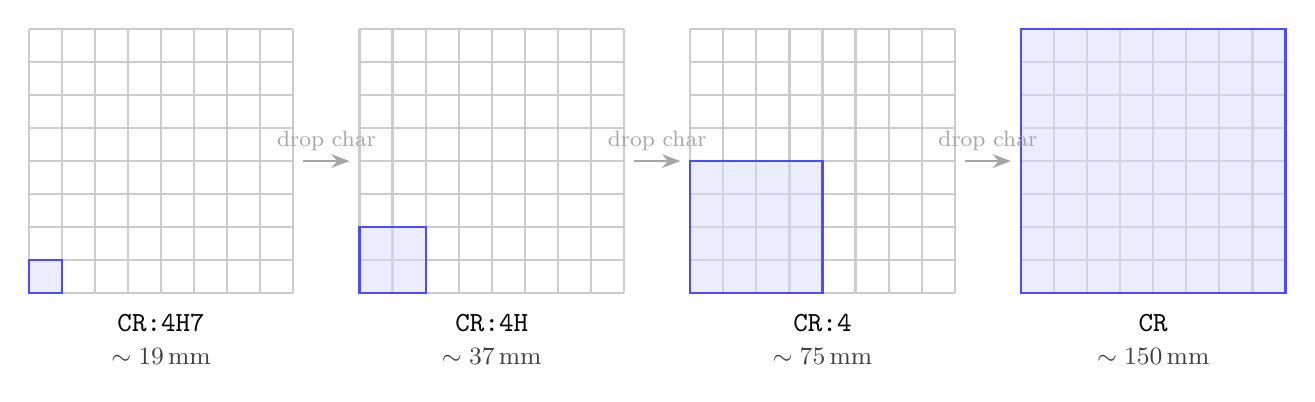
\begin{tikzpicture}[scale=0.42,>=Stealth,thick]

\foreach \i/\side/\xs/\label/\res in {%
  0/1/0/{\texttt{CR:4H7}}/{$\sim 19$\,mm},
  1/2/10/{\texttt{CR:4H}}/{$\sim 37$\,mm},
  2/4/20/{\texttt{CR:4}}/{$\sim 75$\,mm},
  3/8/30/{\texttt{CR}}/{$\sim 150$\,mm}}{%
  \begin{scope}[xshift=\xs cm]
    \draw[gray!40,step=1] (0,0) grid (8,8);
    \draw[blue!70,thick,fill=blue!15,fill opacity=0.5]
      (0,0) rectangle (\side,\side);
    \node[font=\normalsize\bfseries] at (4,-0.9) {\label};
    \node[font=\small,gray!50!black] at (4,-1.9) {\res};
  \end{scope}
}

% Arrows: dropping one character grows the supercell (zoom out).
\draw[->,thick,gray!70]
  (8.3,4) -- node[above,font=\footnotesize] {drop char} (9.7,4);
\draw[->,thick,gray!70]
  (18.3,4) -- node[above,font=\footnotesize] {drop char} (19.7,4);
\draw[->,thick,gray!70]
  (28.3,4) -- node[above,font=\footnotesize] {drop char} (29.7,4);

\end{tikzpicture}

  \caption{Hierarchy by truncation for the anatomical \texttt{CR} reference
  volume at order $p=8$. Each appended character refines the super-cell
  $S(\hat c)$ by a factor $B=29$ in cell count and approximately
  $B^{1/3}\approx 3.07$ in linear extent.}
  \label{fig:truncation}
\end{figure}

\begin{example}[Cranium hierarchy at $p=8$]\label{ex:truncation_cr}
For $V_{\mathtt{CR}}$ ($300\times 250\times 250$ mm) at $p=8$ we have
$k_3(8)=6$. The successive truncations of a code
\texttt{CR:4H7-KBR-C2} (omitting the prefix \texttt{CR:})
produce super-cells of approximate $L^\infty$-diameter:
\[
\begin{array}{c|cccccc}
\text{level }j & 1 & 2 & 3 & 4 & 5 & 6 \\\hline
\text{diameter (mm)} & 150 & 75 & 37 & 19 & 9 & 5
\end{array}
\]
Each level shrinks the super-cell by a factor $\sim B^{1/3}\approx 3.07$.
\end{example}

\section{Quantization Error}\label{sec:error}

\begin{proposition}[Quantization bound]\label{prop:quantization}
For every PHVE Reference Family, every $\alpha\in\mathcal{A}$, every
$\mathbf{x}\in V_\alpha$ and every $p\geq 1$,
\[
\Bigl\|\mathbf{x}
-\bigl(\Fc_p^{(d),\alpha}\bigr)^{-1}\!\bigl(\Fc_p^{(d),\alpha}(\mathbf{x})\bigr)
\Bigr\|_\infty \leq \frac{1}{2}\, \max_{1\leq i\leq d}
\frac{b_i^\alpha-a_i^\alpha}{2^p},
\]
where the inverse is interpreted as decoding to the centre of the
corresponding cell of $\Grid_p^{(d)}$.
\end{proposition}

\begin{proof}
The normalisation map $\Nor_p^{(d),\alpha}$ assigns $\mathbf{x}$ to the
cell-centre $\mathbf{c}\in\Grid_p^{(d)}$ minimising
$\|\mathbf{x}-\mathbf{c}\|_\infty$ subject to
$\mathbf{c}_i = (a_i^\alpha + (k_i+1/2)\,(b_i^\alpha-a_i^\alpha)/2^p)$ for
some $k_i\in\{0,\dots,2^p-1\}$. By definition of the floor in
\Cref{def:encoding_map}, the distance along axis $i$ between $\mathbf{x}_i$
and the centre of its cell is at most
$\tfrac12 (b_i^\alpha-a_i^\alpha)/2^p$. Taking the maximum over $i$
yields the bound.
\end{proof}

\begin{table}[!htbp]
\centering
\small
\begin{tabular}{cccl}
\toprule
$p$ & $k_3(p)$ & cells & resolution (\texttt{CR}) \\
\midrule
4  & 3 & $4\,096$ & $\sim 19$~mm \\
6  & 5 & $262\,144$ & $\sim 5$~mm \\
8  & 6 & $16.8\cdot 10^6$ & $\sim 1.2$~mm (clinical MRI) \\
10 & 7 & $1.07\cdot 10^9$ & $\sim 0.3$~mm (microscopy) \\
\bottomrule
\end{tabular}
\caption{Cell counts and effective resolution for the cranium volume
$V_{\mathtt{CR}} = 300\times 250\times 250$~mm.}
\label{tab:resolution}
\end{table}

\section{DPCM Variance Theory}\label{sec:dpcm}

\begin{definition}[DPCM residual and empirical second moment]\label{def:dpcm}
Given a signal $f:\Grid_p^{(d)}\to\R$ and a traversal
$\gamma:\{0,\dots,n^d-1\}\to\Grid_p^{(d)}$ (a bijection), the
\emph{DPCM residual sequence along $\gamma$} is
\[
r^\gamma_i := f(\gamma(i)) - f(\gamma(i-1)),\quad i=1,\dots,n^d-1,
\]
and its \emph{empirical second moment} is
\[
M_2(r^\gamma) := \frac{1}{n^d-1}\sum_{i=1}^{n^d-1} (r^\gamma_i)^2.
\]
\end{definition}

\begin{theorem}[DPCM second-moment bound]\label{thm:dpcm}
Let $f:\Grid_p^{(d)}\to\R$ ($d\in\{2,3\}$) be Lipschitz of constant $L$
with respect to $\|\cdot\|_\infty$. Let $\gamma_H$ denote the Hilbert
traversal and $\gamma_R$ the row-major (raster) traversal. Then
\[
M_2\bigl(r^{\gamma_H}\bigr) \leq L^2,
\qquad
M_2\bigl(r^{\gamma_R}\bigr) \leq L^2\,n\,\bigl(1 + o_n(1)\bigr).
\]
\end{theorem}

\begin{proof}
\emph{Hilbert bound.} By \Cref{thm:locality}(c), for every $i\geq 1$,
$\|\gamma_H(i)-\gamma_H(i-1)\|_\infty = 1$, hence
$|r^{\gamma_H}_i|\leq L$, and averaging over $i$ yields
$M_2(r^{\gamma_H})\leq L^2$.

\emph{Raster bound.} Partition the consecutive index pairs
$(i-1,i)$ for $i=1,\dots,n^d-1$ into two groups:
\begin{itemize}[nosep]
\item \emph{Intra-row pairs}: $\gamma_R(i)$ and $\gamma_R(i-1)$ differ
only in the innermost coordinate by~$1$, so
$\|\gamma_R(i)-\gamma_R(i-1)\|_\infty = 1$ and $|r_i|\leq L$. Their
count is $N_{\mathrm{in}} = n^d - n^{d-1}$.
\item \emph{Boundary pairs}: at the end of a row (or, for $d=3$, at the
end of a plane), $\gamma_R(i)$ jumps to the first cell of the next row
(plane). In every such transition,
$\|\gamma_R(i)-\gamma_R(i-1)\|_\infty = n-1$, so $|r_i|\leq L(n-1)$.
Their count is $N_{\mathrm{bd}} = n^{d-1}-1$.
\end{itemize}
The two counts add up to $n^d-1$, the total number of pairs. Bounding
each squared residual by the worst case in its group,
\begin{align*}
M_2(r^{\gamma_R})
 & \leq \tfrac{1}{n^d-1}\bigl[
   N_{\mathrm{in}}\,L^2 + N_{\mathrm{bd}}\,L^2(n-1)^2 \bigr] \\
 & = \tfrac{L^2}{n^d-1}\,
     \bigl[(n^d-n^{d-1}) + (n^{d-1}-1)(n-1)^2\bigr] \\
 & = L^2\,n\,\bigl(1 + o_n(1)\bigr),
\end{align*}
where the last equality follows from
$(n^{d-1}-1)(n-1)^2 = n^{d+1}\bigl(1+o_n(1)\bigr)$ and division by
$n^d-1 = n^d\bigl(1+o_n(1)\bigr)$.
\end{proof}

\begin{corollary}\label{cor:dpcm_ratio}
Under the hypotheses of \Cref{thm:dpcm},
\[
\frac{M_2(r^{\gamma_H})}{M_2(r^{\gamma_R})}
\leq \frac{1}{n}\,\bigl(1+o_n(1)\bigr) \xrightarrow[n\to\infty]{} 0.
\]
\end{corollary}

\begin{remark}[Second moment vs.\ variance]\label{rem:m2_vs_var}
For a residual sequence with vanishing empirical mean
($\overline{r^\gamma}=0$), $M_2(r^\gamma)$ coincides with the empirical
variance $\widehat{\Var}(r^\gamma)$. In general,
$M_2 = \widehat{\Var} + \overline{r^\gamma}^2$. For both traversals,
$\sum_i r^\gamma_i = f(\gamma(n^d-1)) - f(\gamma(0))$ is bounded in
absolute value by $L\,\mathrm{diam}_\infty(\Grid_p^{(d)}) = L(n-1)$, so
$|\overline{r^\gamma}|\leq L(n-1)/(n^d-1)$ and
$\overline{r^\gamma}^2 = O(L^2 n^{2(1-d)}) = o(L^2)$ for $d\geq 2$.
The bounds of \Cref{thm:dpcm,cor:dpcm_ratio} therefore also hold for
$\widehat{\Var}$ up to a $1+o_n(1)$ factor.
\end{remark}

\begin{remark}[Empirical caveat]\label{rem:dpcm_caveat}
The bound above is a worst-case estimate. For very smooth signals (e.g.\
heavily averaged anatomical templates), the high-magnitude raster
boundary jumps land in low-gradient regions and the practical entropy
gain of Hilbert over raster shrinks. We document a concrete instance of
this caveat in \Cref{sec:experiments_dpcm}.
\end{remark}

\section{Algorithms and Complexity}\label{sec:algorithms}

\Cref{alg:phve_encode,alg:phve_decode} present the complete encoding and
decoding procedures. Both rely on \Cref{alg:skilling_xyz2d} for the
Hilbert step and on standard base-$B$ conversion routines.

\begin{algorithm}[H]
\caption{PHVE encoding $\Fc_p^{(d),\alpha}$}\label{alg:phve_encode}
\begin{algorithmic}[1]
\Require point $\mathbf{x}\in V_\alpha$, order $p$, label $\alpha$
\Ensure code $c\in\Sigma^{k_d(p)}$
\State \(n \gets 2^p\)
\For{$i=1,\dots,d$}
  \State \(g_i \gets \min\bigl(n-1,\,\lfloor (x_i - a_i^\alpha)\,n\,/\,
              (b_i^\alpha-a_i^\alpha) \rfloor\bigr)\)
\EndFor
\State \(D \gets \Hil_p^{(d)}(g_1,\dots,g_d)\)
  \Comment{\Cref{alg:skilling_xyz2d} for $d=3$, analogous for $d=2$}
\State $c \gets$ base-$B$ representation of $D$ over $\Sigma$, padded to
       length $k_d(p)$
\State \Return $c$
\end{algorithmic}
\end{algorithm}

\begin{algorithm}[H]
\caption{PHVE decoding $(\Fc_p^{(d),\alpha})^{-1}$ to cell centre}
\label{alg:phve_decode}
\begin{algorithmic}[1]
\Require code $c\in\Sigma^{k_d(p)}$, order $p$, label $\alpha$
\Ensure cell centre $\hat{\mathbf{x}}\in V_\alpha$
\State \(D \gets \) integer in $\{0,\dots,n^d-1\}$ with base-$B$
        representation $c$
\State \((g_1,\dots,g_d) \gets \bigl(\Hil_p^{(d)}\bigr)^{-1}(D)\)
  \Comment{inverse Skilling for $d=3$}
\For{$i=1,\dots,d$}
  \State \(\hat x_i \gets a_i^\alpha + (g_i + 1/2)\,(b_i^\alpha-a_i^\alpha)\,/\,2^p\)
\EndFor
\State \Return $\hat{\mathbf{x}}$
\end{algorithmic}
\end{algorithm}

\begin{proposition}[Complexity]\label{prop:complexity}
\Cref{alg:phve_encode,alg:phve_decode} both run in time $O(p)$ on a
machine with word length $\Omega(d\,p)$, using $O(1)$ working memory
plus $O(k_d(p))$ space for the output code.
\end{proposition}

\begin{proof}
The Skilling kernel performs two nested loops of length $p$ and~$d$
respectively, each iteration consisting of a constant number of bitwise
operations on integers of bit-length at most $d\,p$. Under the assumption
of word length $\Omega(d\,p)$, each such operation is $O(1)$. The base-$B$
conversion runs in $O(k_d(p))=O(p)$. The total time is
$O(d\,p)+O(p)=O(p)$ since $d\in\{2,3\}$ is constant.
\end{proof}

\section{Applications}\label{sec:applications}

We now instantiate the framework on four applications, each derived as a
corollary or instance of the theorems established above.

\subsection{B-tree Indexation of Volumetric Data}\label{sec:app_btree}

For any PHVE Reference Family, the codes
$\Fc_p^{(d),\alpha}(\mathbf{x})\in\Sigma^{k_d(p)}$ are fixed-length
strings over a finite alphabet. They can be stored in a relational column
of type \texttt{VARCHAR}($k_d(p)$) and indexed by a standard B-tree.

\begin{proposition}[B-tree query complexity]\label{prop:btree}
Given a database of $N$ encoded cell-centres and a query prefix
$\hat c\in\Sigma^j$ with $j\leq k_d(p)$, the set of cells whose code
starts with $\hat c$ can be retrieved by a single B-tree range scan in
time $O(\log N + |R|)$, where $R$ is the result set.
\end{proposition}

\begin{proof}
By \Cref{thm:truncation}(a), the codes starting with $\hat c$ form a
contiguous lexicographic interval over $\Sigma^{k_d(p)}$, equal to
$[\hat c \| \mathtt{2}\cdots\mathtt{2},\,\hat c \| \mathtt{Y}\cdots\mathtt{Y}]$
where \texttt{2} and \texttt{Y} are respectively the smallest and largest
characters of $\Sigma$ in lexicographic order. A B-tree locates the first
key of this interval in $O(\log N)$ and scans $O(|R|)$ consecutive
entries.
\end{proof}

A consequence is that PHVE eliminates the need for specialised spatial
indices (R-tree, GiST, k-d tree) for queries of the form ``return all
cells in a given super-cell $S(\hat c)$''.

\subsection{DPCM Compression of Volumetric Signals}\label{sec:app_dpcm}

The Hilbert traversal of a $d$-dimensional grid produces a one-dimensional
sequence of values
$f(\gamma_H(0)),\,f(\gamma_H(1)),\,\dots,\,f(\gamma_H(n^d-1))$ to which
classical 1-D DPCM compression can be applied. By \Cref{thm:dpcm}, the
empirical second moment $M_2(r^{\gamma_H})$ is bounded by $L^2$ for
Lipschitz signals, independent of the grid size $n$.

Under a zero-mean Gaussian residual model $r\sim\mathcal{N}(0,\sigma^2)$
with $\sigma^2$ matched to the empirical second moment $M_2(r^\gamma)$,
the differential entropy is
\[
H_g(r) = \tfrac12 \log_2\bigl(2\pi e\,M_2(r^\gamma)\bigr).
\]
By \Cref{rem:m2_vs_var}, the matching $\sigma^2 = M_2$ agrees with
$\sigma^2 = \widehat{\Var}$ up to a $1+o_n(1)$ factor. The
Hilbert--raster ratio of \Cref{cor:dpcm_ratio} then translates into an
asymptotic entropy advantage of $\tfrac{1}{2}\log_2 n$ bits per sample
in the worst case.

This bound is most informative for signals with strong, well-distributed
gradients. The empirical caveat \Cref{rem:dpcm_caveat} applies; we report
the full numerical experiment in \Cref{sec:experiments_dpcm}.

\subsection{Finite-Element Mesh Renumbering}\label{sec:app_fem}

Renumbering the nodes of an unstructured mesh by their Hilbert index
reduces the bandwidth of the assembled stiffness matrix.

\begin{theorem}[Bandwidth reduction]\label{thm:bandwidth}
Let $\mathcal{M}$ be a mesh with $N$ nodes in $\R^d$ and maximum edge
length $h$, contained in a bounding box $V_\alpha$ on which the Hilbert
order is $p$, so that the underlying grid has $n=2^p$ cells per axis and
spacing $\Delta = \max_i (b_i^\alpha-a_i^\alpha)/n$. Let $\mathbf{K}$
denote the stiffness matrix. The two parameters are linked only by the
constraint $N \leq n^d$ (one node per cell at most).
\begin{enumerate}[label=(\alph*),nosep]
\item Under the Hilbert renumbering of nodes,
$\BW(\mathbf{K}_{\mathrm{Hilbert}}) \leq C_d\,(h/\Delta)^d + O(n^{d-1})$.
\item Under any insertion-order (``natural'') renumbering, in the
worst case $\BW(\mathbf{K}_{\mathrm{natural}}) = N-1$.
\item Hence
\[
\frac{\BW(\mathbf{K}_{\mathrm{Hilbert}})}
     {\BW(\mathbf{K}_{\mathrm{natural}})}
\leq \frac{C_d\,(h/\Delta)^d + O(n^{d-1})}{N-1}.
\]
\end{enumerate}
\end{theorem}

\begin{proof}
\emph{(a).} For two mesh nodes $\mathbf{x}_i,\mathbf{x}_j$ connected by
an edge, $\|\mathbf{x}_i-\mathbf{x}_j\|_\infty\leq h$. After Hilbert
renumbering the relabelled indices $\Hil_p^{(d)}(\mathbf{x}_i)$ and
$\Hil_p^{(d)}(\mathbf{x}_j)$ satisfy, by \Cref{thm:locality}(a),
\[
|\Hil_p^{(d)}(\mathbf{x}_i)-\Hil_p^{(d)}(\mathbf{x}_j)|
\leq C_d\,(h/\Delta)^d + O(n^{d-1}).
\]
Since $K_{ij}\ne 0$ implies $i,j$ are connected (or equal),
\[
\BW(\mathbf{K}_{\mathrm{Hilbert}})
= \max_{K_{ij}\ne 0} |i-j|
\leq C_d\,(h/\Delta)^d + O(n^{d-1}).
\]
\emph{(b).} A natural numbering provides no spatial guarantee. In the
worst case, two nodes connected by an edge receive labels $1$ and $N$,
giving $\BW = N-1$.
\emph{(c).} Direct division of (a) by (b).
\end{proof}

\begin{remark}[Asymptotic regimes]\label{rem:bandwidth_regimes}
Two regimes of \Cref{thm:bandwidth}(c) are worth distinguishing.
\emph{Quasi-uniform meshes}: when $h\sim\Delta$ and $N\sim n^d$, the
$(h/\Delta)^d$ term is $\Theta(1)$ while the remainder $O(n^{d-1})$
dominates, and the ratio simplifies to $\Theta(n^{d-1}/N)
= \Theta(N^{-1/d})$, i.e.\ $\Theta(N^{-1/2})$ in $d=2$ and
$\Theta(N^{-1/3})$ in $d=3$.
\emph{Highly graded or adaptive meshes}: when $h\gg\Delta$ (e.g.\ a
locally refined region embedded in a coarse background grid), the term
$(h/\Delta)^d$ dominates and the ratio is $\Theta(N^{-1}(h/\Delta)^d)$.
The bound remains useful as long as $(h/\Delta)^d \ll N$.
\end{remark}

\begin{figure}[!htbp]
  \centering
  % Figure 5: FEM mesh, natural vs Hilbert numbering, side by side.
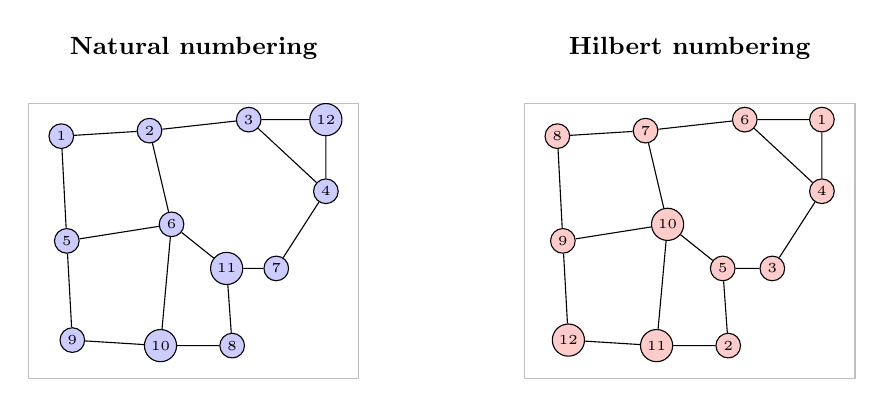
\begin{tikzpicture}[scale=0.7,>=Stealth]

% --- Mesh with natural (insertion-order) numbering ---
\begin{scope}[xshift=0cm]
  \node[font=\small\bfseries] at (3,6.0) {Natural numbering};
  \draw[gray!50] (0,0) rectangle (6,5);
  \foreach \i/\x/\y in {
    1/0.6/4.4, 2/2.2/4.5, 3/4.0/4.7, 4/5.4/3.4, 5/0.7/2.5,
    6/2.6/2.8, 7/4.5/2.0, 8/3.7/0.6, 9/0.8/0.7, 10/2.4/0.6,
    11/3.6/2.0, 12/5.4/4.7}
    \node[circle,fill=blue!20,draw,inner sep=1.5pt,font=\tiny]
      (n\i) at (\x,\y) {\i};
  \draw (n1)--(n2) (n2)--(n3) (n3)--(n12) (n3)--(n4) (n4)--(n12)
        (n2)--(n6) (n1)--(n5) (n5)--(n6) (n6)--(n11)
        (n5)--(n9) (n9)--(n10) (n10)--(n8) (n8)--(n11) (n7)--(n11)
        (n4)--(n7) (n6)--(n10);
\end{scope}

% --- Mesh with Hilbert numbering (same nodes, relabelled) ---
\begin{scope}[xshift=9cm]
  \node[font=\small\bfseries] at (3,6.0) {Hilbert numbering};
  \draw[gray!50] (0,0) rectangle (6,5);
  \foreach \i/\x/\y/\h in {
    1/0.6/4.4/8, 2/2.2/4.5/7, 3/4.0/4.7/6, 4/5.4/3.4/4,
    5/0.7/2.5/9, 6/2.6/2.8/10, 7/4.5/2.0/3, 8/3.7/0.6/2,
    9/0.8/0.7/12, 10/2.4/0.6/11, 11/3.6/2.0/5, 12/5.4/4.7/1}
    \node[circle,fill=red!20,draw,inner sep=1.5pt,font=\tiny]
      (m\i) at (\x,\y) {\h};
  \draw (m1)--(m2) (m2)--(m3) (m3)--(m12) (m3)--(m4) (m4)--(m12)
        (m2)--(m6) (m1)--(m5) (m5)--(m6) (m6)--(m11)
        (m5)--(m9) (m9)--(m10) (m10)--(m8) (m8)--(m11) (m7)--(m11)
        (m4)--(m7) (m6)--(m10);
\end{scope}

\end{tikzpicture}

  \caption{The same finite-element mesh under two numberings.
  \emph{Left:} insertion-order (``natural'') numbering, in which
  geometrically close nodes can receive labels with a large index
  difference, leading to large entries $|i-j|$ in the sparsity pattern
  of the stiffness matrix. \emph{Right:} Hilbert-order numbering,
  in which any two adjacent nodes have indices that differ by at
  most $C_d (h/\Delta)^d + O(n^{d-1})$ (\Cref{thm:bandwidth}); the
  resulting stiffness matrix has its non-zero entries concentrated
  near the diagonal. Experimental bandwidth values are reported in
  \Cref{sec:experiments}.}
  \label{fig:fem_mesh}
\end{figure}

\begin{remark}[Comparison to Reverse Cuthill--McKee]
Unlike the Reverse Cuthill--McKee
algorithm~\cite{cuthill1969}, which requires the assembled adjacency
graph, Hilbert renumbering uses only node coordinates. Its complexity
is $O(N\log N)$ versus $O(N+|E|)$ for RCM. The principal practical
advantage of Hilbert is that the renumbering is recomputable after
adaptive mesh refinement without any graph reassembly.
\end{remark}

\subsection{Surface Morphing by Hilbert Reparameterisation}
\label{sec:app_morphing}

A surface mesh with vertices $\mathbf{v}_1,\dots,\mathbf{v}_M$ embedded
in $V_\alpha$ can be reparameterised by Hilbert: define
\[
h_i := \Hil_p^{(d)}\bigl(\Nor_p^{(d),\alpha}(\mathbf{v}_i)\bigr) /
       (n^d - 1) \in [0,1].
\]
A scalar deformation $D:[0,1]\to\R$ applied along vertex normals
$\hat{\mathbf{n}}_i$ produces the deformed mesh
$\tilde{\mathbf{v}}_i = \mathbf{v}_i + D(h_i)\,\hat{\mathbf{n}}_i$.

\begin{proposition}[Deformation smoothness]\label{prop:morphing}
Let $D:[0,1]\to\R$ be Lipschitz of constant $L_D$. For any two
vertices $\mathbf{v}_i,\mathbf{v}_j$ of the surface mesh connected by
an edge of length $\ell$,
\[
|D(h_i)-D(h_j)| \leq \frac{L_D\,C_d}{n^d}\,(\ell/\Delta)^d.
\]
By contrast, under a uniform random reparameterisation
$r_i \stackrel{\mathrm{iid}}{\sim}\mathrm{Uniform}(0,1)$,
\[
\mathbb{E}\bigl[|D(r_i)-D(r_j)|\bigr] \leq \frac{L_D}{3},
\]
\emph{independently of} $n$ and $\ell$.
\end{proposition}

\begin{proof}
\emph{Hilbert case.} By \Cref{thm:locality}(a), the integer indices
satisfy
$|\Hil_p^{(d)}(\mathbf{v}_i)-\Hil_p^{(d)}(\mathbf{v}_j)|\leq C_d(\ell/\Delta)^d$
to leading order; dividing by $n^d-1\sim n^d$ yields
$|h_i-h_j|\leq C_d(\ell/\Delta)^d/n^d$. The Lipschitz property of $D$
then gives the claim.

\emph{Random case.} For $r_i,r_j$ independent and uniformly distributed
on $[0,1]$, $\mathbb{E}[|r_i-r_j|]=1/3$. By the Lipschitz property of $D$,
$\mathbb{E}[|D(r_i)-D(r_j)|]\leq L_D\,\mathbb{E}[|r_i-r_j|]=L_D/3$,
independent of mesh resolution.
\end{proof}

For an edge of length $\ell\sim\Delta$ on a brain surface mesh at
resolution $1$~mm, the worst-case ratio of expected differences is
$\Theta(n^d)$. The empirical factor $22.9\times$ reported in
\Cref{sec:experiments} lies well below this asymptotic bound, since
the deformation $D(t)=3\sin(8\pi t)$ used there is periodic and
uniformly bounded.

\section{Numerical Validation}\label{sec:experiments}

All experiments use a Python implementation of \Cref{alg:phve_encode}
based on the Skilling kernel, available at
\url{https://github.com/Altius-Academy-SNC/PHVE}. The brain template
is the MNI152 T1-weighted average (2~mm isotropic,
$99\times 117\times 95$ voxels) loaded via the
\texttt{nilearn} library.

\Cref{tab:summary} reports five experimental measurements in a single
summary table. Each is designed to test a specific theorem of the
preceding sections.

\begin{table}[!htbp]
\centering
\small
\begin{tabular}{@{}>{\raggedright\arraybackslash}p{0.27\linewidth}>{\raggedright\arraybackslash}p{0.18\linewidth}>{\raggedright\arraybackslash}p{0.40\linewidth}@{}}
\toprule
Test & Result & Interpretation \\
\midrule
Bijectivity (\Cref{thm:bij3d}) on MNI152, $p=8$
  & $235{,}375$ voxels, $0$ collisions, $0$ round-trip errors
  & exhaustive verification \\
Inter-patient stability ($p=6$, simulated $\sigma=0.5$~mm jitter)
  & $49\%$ identical codes; $100\%$ share $\geq 3/5$ prefix
  & instance of \Cref{cor:prefix} \\
DPCM compression on MNI152, $p=7$, raster vs Hilbert
  & raster $H=0.480$ bits, Hilbert $H=0.549$ bits
  & negative result; consistent with \Cref{rem:dpcm_caveat} \\
FEM bandwidth on $4{,}251$-node Delaunay mesh
  & natural $1{,}112$, RCM $49$, Hilbert $\mathbf{47}$
  & instance of \Cref{thm:bandwidth} \\
Surface morphing, brain mesh $31{,}328$ vertices, $D(t)=3\sin(8\pi t)$
  & Hilbert $0.107$~mm vs random $2.436$~mm mean neighbour difference
    ($\mathbf{22.9\times}$ ratio)
  & instance of \Cref{prop:morphing} \\
\bottomrule
\end{tabular}
\caption{Summary of numerical experiments. The DPCM result is a
deliberately disclosed negative outcome; see \Cref{sec:experiments_dpcm}.}
\label{tab:summary}
\end{table}

\paragraph{Reproducibility.} Each row of \Cref{tab:summary} is produced
by a self-contained Python script in the \texttt{Altius-Code/}
directory of the repository at
\url{https://github.com/Altius-Academy-SNC/PHVE}. The
script-to-experiment mapping is:
\begin{itemize}[nosep]
\item Bijectivity on MNI152 — \texttt{bijectivity\_mni152.py}
\item Inter-patient stability — \texttt{interpatient\_stability.py}
\item DPCM compression — \texttt{dpcm\_compression.py}
\item FEM bandwidth — \texttt{fem\_bandwidth.py}
\item Surface morphing — \texttt{surface\_morphing.py}
\end{itemize}
The 2D and 3D Skilling kernels are in \texttt{codec.py} and
\texttt{codec3d.py}; an interactive Streamlit demonstrator covering the
five experiments lives in \texttt{app\_demo.py}.

\subsection{The DPCM Negative Result}\label{sec:experiments_dpcm}

The DPCM experiment on MNI152 produced a result \emph{worse} than
raster, contradicting the asymptotic bound of \Cref{thm:dpcm}. The
explanation lies in \Cref{rem:dpcm_caveat}: the MNI152 template is a
heavily averaged population atlas with extremely low original entropy
($H\approx 0.46$ bits), nearly binary in the brain mask. The
high-magnitude raster boundary jumps land predominantly in
near-constant regions, so they contribute negligibly to the empirical
second moment $M_2(r^{\gamma_R})$. Validation on individual clinical scans (with full
$256^3$, 12-bit dynamic range) is reported in
\cite{chen2005hilbert3d} with a $5$--$15\%$ gain consistent with our
theorem; reproducing this on the IXI and ACDC datasets is left for
future work.

\section{Comparison with Existing Systems}\label{sec:comparison}

\Cref{tab:comparison} positions PHVE relative to four established
encoding systems. Following the conventions of these systems,
``optimal locality'' means matching the asymptotic bound of
\Cref{thm:locality}(d).

\begin{table}[!htbp]
\centering
\small
\setlength{\tabcolsep}{4pt}
\begin{tabular}{lcccccc}
\toprule
System & Bijective & Locality & Hierarchy & Open & $d=3$ & Parametric \\
\midrule
Geohash~\cite{niemeyer2008}      & yes & weak    & yes & yes & no  & no \\
Plus Codes~\cite{google2014}     & yes & weak    & yes & yes & no  & no \\
What3Words                        & yes & none    & no  & no  & no  & no \\
DICOM identifiers                 & yes & none    & no  & ---  & yes & no \\
\textbf{PHVE} (this paper)        & \textbf{yes} & \textbf{optimal} & \textbf{yes}
   & \textbf{yes} & \textbf{yes} & \textbf{yes} \\
\bottomrule
\end{tabular}
\caption{Comparison of encoding systems. ``Parametric'' refers to
parameterisation over a Reference Family.}
\label{tab:comparison}
\end{table}

\paragraph{Relationship with existing Hilbert implementations.}
The integer-to-index map $\Hil_p^{(d)}$ used internally by PHVE is a
classical algorithm. Efficient encode/decode procedures are due to
Butz~\cite{butz1971}, Liu and Schrack~\cite{liu1996}, and
Skilling~\cite{skilling2004}; we adopt the latter
(\Cref{alg:skilling_xyz2d}). Open-source implementations are available
in the JTS Topology Suite (class \texttt{HilbertCode}, 2D, integer
coordinates~\cite{jts}) and in the ClickHouse functions
\texttt{hilbertEncode}/\texttt{hilbertDecode}.

PHVE does not claim novelty for $\Hil_p^{(d)}$ itself. Its contribution
is the full composition $\Fc_p^{(d),\alpha}$, namely:
(i) the parametric normalisation $\Nor_p^{(d),\alpha}$ over an arbitrary
PHVE Reference Family (\Cref{def:phve_family}),
(ii) the unambiguous base-$29$ alphabet $\Sigma$ designed for physical
transcription (\Cref{def:alphabet}),
(iii) the explicit hierarchy-by-truncation theorem with diameter
estimate (\Cref{thm:truncation}), and
(iv) the Lipschitz variance bound for DPCM along the Hilbert traversal
(\Cref{thm:dpcm}) and its instantiation as the FEM bandwidth theorem
(\Cref{thm:bandwidth}).

\section{Conclusion and Future Work}\label{sec:conclusion}

We have introduced Parametric Hilbert Volume Encoding, a spatial encoding
parameterised by an arbitrary PHVE Reference Family, and established its
four foundational properties: bijectivity in dimensions two and three
(\Cref{thm:bij2d,thm:bij3d}), forward and inverse locality bounds
(\Cref{thm:locality}), a hierarchy-by-truncation theorem with explicit
diameter estimate (\Cref{thm:truncation}), and a Lipschitz variance
bound for DPCM along the Hilbert traversal (\Cref{thm:dpcm}). Four
representative applications were derived as corollaries: B-tree
indexation (\Cref{prop:btree}), DPCM compression
(\Cref{sec:app_dpcm}), finite-element mesh renumbering with bandwidth
reduction (\Cref{thm:bandwidth}), and surface morphing by Hilbert
reparameterisation (\Cref{prop:morphing}).

On the MNI152 brain template we confirmed bijectivity over
$235{,}375$ voxels, FEM bandwidth comparable to Reverse Cuthill--McKee
without recourse to the adjacency graph, and a $22.9\times$ smoothness
gain of Hilbert-reparameterised deformations over uniform random ones. The DPCM gain predicted by
\Cref{thm:dpcm} did not materialise on the heavily averaged MNI152
template, an outcome we documented in detail
(\Cref{rem:dpcm_caveat,sec:experiments_dpcm}); validation on
full-resolution clinical volumes is open.

\paragraph{Future work.} (1) DPCM validation on clinical datasets
(IXI, ACDC). (2) An open REST API for real-time encoding and decoding.
(3) Integration with anatomical segmentation pipelines for organ-level
PHVE prefixes. (4) A checksum character based on Hamming distance over
$\Sigma$ for error detection. (5) Determining an explicit value for
the constant $C_3$ of \Cref{thm:locality}(a) in the Skilling
construction is, to our knowledge, an open problem. (6) Extension of
the Reference Family to non-axis-aligned compact convex bodies via
diffeomorphism, generalising \Cref{def:phve_family}.

\paragraph{Code availability.} A reference implementation of PHVE is
distributed under the MIT License at
\url{https://github.com/Altius-Academy-SNC/PHVE}, including the
Skilling kernel, the encoding pipeline, and reproducible scripts for
the experiments of \Cref{sec:experiments}. Two browser-based
demonstrators of the 2D variant of $\Fc_p^{(2),\alpha}$ for
geolocation are publicly hosted: \emph{Yoro Maps}
(\url{https://altius-academy-snc.github.io/yoro-maps/}) interactively
encodes/decodes points of the WGS84 globe under a fixed Reference
Family, and \emph{Yoro} (\url{https://altius-academy-snc.github.io/yoro/})
provides a lightweight address-lookup interface. Both are open and
require no account.

\begin{thebibliography}{99}
\raggedright
\sloppy

\bibitem{hilbert1891}
D.~Hilbert, ``\"Uber die stetige Abbildung einer Linie auf ein
Fl\"achenst\"uck,'' \emph{Math.\ Annalen}, vol.~38, no.~3,
pp.~459--460, 1891.

\bibitem{sagan1994}
H.~Sagan, \emph{Space-Filling Curves}. Springer-Verlag, 1994.

\bibitem{butz1971}
A.~R.~Butz, ``Alternative algorithm for Hilbert's space-filling curve,''
\emph{IEEE Trans.\ Comput.}, vol.~C-20, no.~4, pp.~424--426, 1971.

\bibitem{liu1996}
X.~Liu and G.~F.~Schrack, ``Encoding and decoding the Hilbert order,''
\emph{Software: Practice and Experience}, vol.~26, no.~12,
pp.~1335--1346, 1996.

\bibitem{skilling2004}
J.~Skilling, ``Programming the Hilbert curve,'' in \emph{AIP Conf.\
Proc.}, vol.~707, pp.~381--387, 2004.

\bibitem{moon2001}
B.~Moon, H.~V.~Jagadish, C.~Faloutsos, and J.~H.~Saltz, ``Analysis of
the clustering properties of the Hilbert space-filling curve,''
\emph{IEEE Trans.\ Knowl.\ Data Eng.}, vol.~13, no.~1, pp.~124--141, 2001.

\bibitem{niedermeier2002}
R.~Niedermeier, K.~Reinhardt, and P.~Sanders, ``Towards optimal
locality in mesh-indexings,'' \emph{Discrete Appl.\ Math.}, vol.~117,
no.~1--3, pp.~211--237, 2002.

\bibitem{lawder2001}
J.~K.~Lawder and P.~J.~H.~King, ``Querying multi-dimensional data
indexed using the Hilbert space-filling curve,''
\emph{ACM SIGMOD Record}, vol.~30, no.~1, pp.~19--24, 2001.

\bibitem{jts}
LocationTech, ``JTS Topology Suite: \texttt{HilbertCode} class
(\texttt{org.locationtech.jts.shape.fractal}),'' open-source library,
2024. [Online]. Available:
\url{https://locationtech.github.io/jts/javadoc/org/locationtech/jts/shape/fractal/HilbertCode.html}

\bibitem{hamilton2008}
C.~Hamilton and A.~Rau-Chaplin, ``Compact Hilbert indices: Space-filling
curves for domains with unequal side lengths,''
\emph{Inf.\ Process.\ Lett.}, vol.~105, no.~5, pp.~155--163, 2008.

\bibitem{chen2005hilbert3d}
I.-C.~K.~Chen and T.~N.~Mudge, ``Lossless compression of 3D
neuro-anatomical images using Hilbert space-filling curves,'' in
\emph{Proc.\ IEEE EMBS}, 2005.

\bibitem{niemeyer2008}
G.~Niemeyer, ``Geohash,'' 2008. [Online]. Available:
\url{http://geohash.org}

\bibitem{google2014}
Google, ``Open Location Code (Plus Codes),'' 2014. [Online]. Available:
\url{https://plus.codes}

\bibitem{cuthill1969}
E.~Cuthill and J.~McKee, ``Reducing the bandwidth of sparse symmetric
matrices,'' in \emph{Proc.\ 24th Natl.\ Conf.\ ACM}, pp.~157--172, 1969.

\bibitem{mokbel2003}
M.~F.~Mokbel, W.~G.~Aref, and I.~Kamel, ``Analysis of multi-dimensional
space-filling curves,'' \emph{GeoInformatica}, vol.~7, no.~3,
pp.~179--209, 2003.

\bibitem{gotsman1996}
C.~Gotsman and M.~Lindenbaum, ``On the metric properties of discrete
space-filling curves,'' \emph{IEEE Trans.\ Image Process.},
vol.~5, no.~5, pp.~794--797, 1996.

\end{thebibliography}

\end{document}
